\documentclass{llncs}

\usepackage{amsmath}
\usepackage{amssymb}
\usepackage{textpos}
\usepackage{graphicx}

\usepackage{style/utils}
\usepackage{style/names}

% -----------------------------------------------------------------------------
\begin{document}

\title		{Witnessing Purity, Constancy and Mutability}
\author		{Ben Lippmeier}
\institute	{School of Computer Science \\ 
		 Australian National University \\
		 \email{Ben.Lippmeier@anu.edu.au}}
\maketitle


% -- Abstract -----------------------------------------------------------------
\begin{abstract}
Restricting destructive update to values of a distinguished reference type prevents functions from being polymorphic in the mutability of their arguments. This restriction makes it easier to reason about program behaviour during transformation, but the lack of polymorphism reduces the expressiveness of the language. We present a System-F style core language that uses dependently kinded proof witnesses to encode information about the mutability of values and the purity of computations. We support mixed strict and lazy evaluation, and use our type system to ensure that only computations without visible side effects are suspended.

\end{abstract}

% -- Intro --------------------------------------------------------------------
\section{Introduction}
\label{Introduction}

Suppose we are writing a library that provides a useful data structure such as linked lists. A Haskell-style definition for the list type would be:
\begin{tabbing}
MM \= MMMMM \= M \= MMMMM \= MMMM \kill
	\> $\kdata \ \iList \ a = \iNil \ | \ \iCons \ a \ (\iList \ a)$
\end{tabbing}

The core language of compilers such as GHC is based around System-F \cite{sulzmann:system-Fc}. Here is the translation of the standard $\imap$ function to this representation, complete with type abstractions and applications:

\begin{tabbing}
MM \= MMM \= MM \= MMMMM \= MMMM \kill
	\> $\imap :: \forall a \ b. \ (a \to b) \to \iList \ a \to \iList \ b$ \\
	\> $\imap = \Lambda a. \ \Lambda b. \ \lambda (f : a \to b). \ \lambda (\ilist : \iList \ a).$ \\
	\> \> $\kcase \ \ilist \ \kof$ \\
	\> \> \> $\iNil$		\> $\to \iNil \ b$ \\
	\> \> \> $\iCons \ x \ \ixs$	\> $\to \iCons \ b \ (f \ x) \ (\imap  \ a \ b \ f \ \ixs)$ 
\end{tabbing}

Say we went on to define some other useful list functions, and then decided that we need one to destructively insert a new element into the middle of a list. In Haskell, side effects are carefully controlled and we would need to introduce a monad such as ST or IO \cite{launchbury:lazy-functional-state-threads} to encapsulate the effects due to the update. Destructive update is also limited to distinguished types such as $\iSTRef$ and $\iIORef$.  We cannot use our previous list type, so will instead change it to use an $\iIORef$.

\begin{tabbing}
MM \= MMMMM \= M \= MMMMM \= MMMM \kill
	\> $\kdata \ \iList \ a = \iNil \ | \ \iCons \ a \ (\iIORef \ (\iList \ a))$
\end{tabbing}

Unfortunately, as we have changed the structure of our original data type, we can no longer use the previous definition of $\imap$, or any other functions we defined earlier. We must go back and refactor each of these function definitions to use the new type. We must insert calls to $\ireadIORef$ and use monadic sequencing combinators instead of vanilla let and where-expressions. However, doing so introduces explicit data dependencies into the core program. This in turn reduces the compiler's ability to perform optimisations such as deforestation and the full laziness transform \cite{santos:compilation}, which require functions to be written in the ``pure'', non-monadic style. It appears that we need \emph{two} versions of our list structure and its associated functions, an immutable version that can be optimised, and a mutable one that can be updated. 

Variations of this problem are also present in ML and O'Caml. In ML, mutability is restricted to $\iref$ and $\iarray$ types \cite{macqueen:sml}. In O'Caml, record types can have mutable fields, but variant types cannot \cite{leroy:ocaml-3.11}. Similarly to Haskell, in these languages we are forced to insert explicit reference types into the definitions of mutable data structures, which makes them incompatible with the standard immutable ones. This paper shows how to avoid this problem:


\begin{itemize}
\item	We present a System-F style core language that uses region and effect typing to guide program optimisation. Optimisations that depend on purity can be performed on the the pure fragments of the program. 
\medskip

\item	We use region variables and dependently kinded witnesses to encode mutability polymorphism. This allows arbitrary data structures to be mutable without changing the structure of their value types.
\medskip

\item	We use call-by-value evaluation as default, but support lazy evaluation via a primitive $\isuspend$ operator. We use witnesses of purity to ensure that only pure function applications can be suspended.
\end{itemize}

Our goals are similar to those of Benton and Kennedy \cite{benton:monads-effects-transformations}, but as in \cite{sulzmann:system-Fc} we use a System-F based core language instead of a monadic one. Type inference and translation from source to core is discussed in \cite{lippmeier:impure-world}.







% --------------------
\section{Why destructive update matters}
\label{intro:update}

Destructive update is the process of changing the value of an object in-place, by overwriting and hence destroying its old value. Without destructive update we cannot change the values of existing objects, only allocate new ones. 

With deference to Turing completeness, destructive update is \emph{simply not required} to write programs. Likewise, almost every feature of a particular language can be shown to be superfluous. Tiny systems such as the Lambda Calculus, Conway's game of life, and the Rule 30 cellular automata are Turing complete~\cite{rendell:life, cook:universal}, and hence capable of universal computation. On the other hand, no one writes programs in them, at least not directly.

When considering language features we must always start from a practical, and therefore subjective viewpoint. When we say ``destructive update matters", we mean that a large enough subset of programmers find it useful that it warrants consideration by all.

We suggest that destructive update furnishes the programmer with two important and powerful tools, and that these tools are either too cumbersome or too inefficient to create without it. The first tool is a set of efficient array-like data structures for managing collections of objects, and the second is the ability to broadcast a new value to all parts of a program with minimal burden on the programmer.


% --------------------
\subsection{Efficient data structures require destructive update}
For a mechanical device such as an internal combustion engine, efficiency is defined as the ratio of useful work output to the amount of energy input to the device~\cite{giancoli:efficiency}. For a \emph{computational} device such as a collection structure, we could reasonably define its efficiency as being the number of insert and update operations that can be completed per hardware clock cycle. 

We pay no attention to the difficulty of designing the structure in the first place. Like internal combustion engines, the development of common data structures is best left to teams of experts, permitting the end user to focus on their own specific tasks.

When the number of objects to be managed is known beforehand, the simplest collection structure is the array. In a typical garbage collected runtime system, the allocation of an array requires just three machine instructions. We test the top-of-heap pointer to ensure enough space is available, write the object header word, and then advance the pointer. The update of a particular value is also straightforward. Suppose we have three registers: R1 holding a pointer to the array, R2 holding the new value, and R3 holding the index of the value to be updated. Many processors can perform this update with just one or two instructions~\cite{sun:sparc-assembly, intel:instruction-set}.

\begin{center}
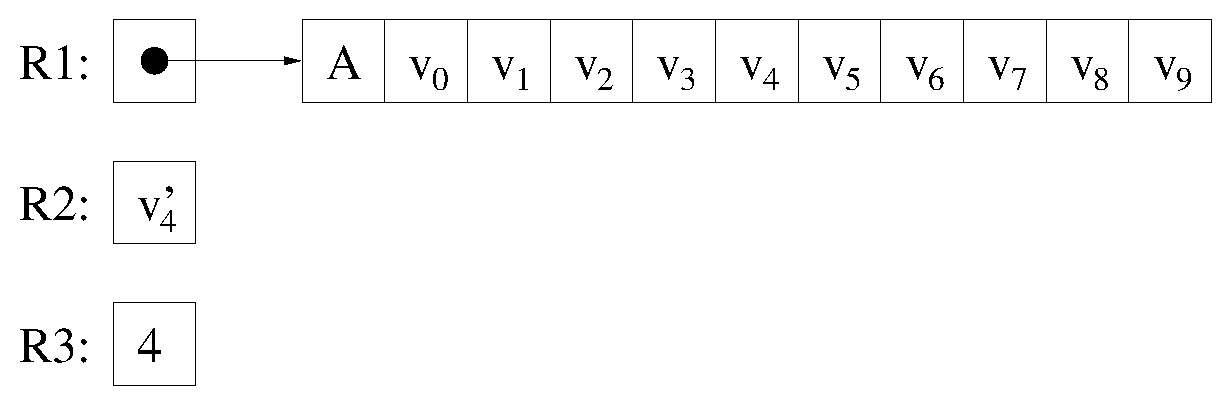
\includegraphics[scale=0.5]{1-Introduction/fig/destructive/data-array10}
\end{center}

Of course, due to pipelining and cache effects, the number of machine instructions executed for an operation does not relate directly to the number of clock cycles used~\cite{hennessy:computer-architecture}. However, it is a usable approximation for this discussion, and we will consider the case of updating a flat array as approaching 100\% efficiency for array-like structures.

Perfect efficiency would be achieved if every update operation completed in the minimum number of clock cycles possible on the available hardware. For most applications, perfect efficiency is unlikely to ever be achieved by a statically compiled program, as it is too difficult to accurately simulate pipeline states and data hazards in a multi-tasking system. 

Ignoring cache effects, the efficiency of an array is independent of how many elements it containts. It costs no more to update a value in a 1000 element array than to update one in a 10 element array.


% --------------------
\subsubsection{Functional arrays are unacceptably slow}
Without destructive update we cannot change an array object once it is allocated, but we can side-step this problem by creating a new object instead of updating the old one. A simple method is to allocate a whole new array and copy the old values into it, with the new value in place of the one that is being updated. This works, but is a disaster for performance. Assuming we need one machine instruction for each value copied, performing an update on a 10 element array now requires 10 instructions, plus three to do the allocation. This represents a miserable 7.7\% efficiency compared with a single instruction destructive update. For a 1000 element array we need at least 1003 instructions, representing approximately 0.1\% efficiency. This is clearly unacceptable.


% --------------------
\subsubsection{Tree structures are only a partial solution}
We can recover some of this ground by using a tree structure instead of a flat array. If we store values in the internal nodes of a balanced binary tree then we need $n$ nodes for $n$ values, and the tree is $\text{ceil} (\log_2(n))$ levels deep. Unfortunately, to change a value in the tree we must still allocate a new node. As this new node will be at a different address from the old one, we must then rebuild all of its parents so that the tree references the new node instead of the old one. For example, in the tree on the next page, to update $v_7$ we must reallocate the node that contains it as well as the nodes of $v_6$, $v_8$ and $v_5$.

\begin{center}
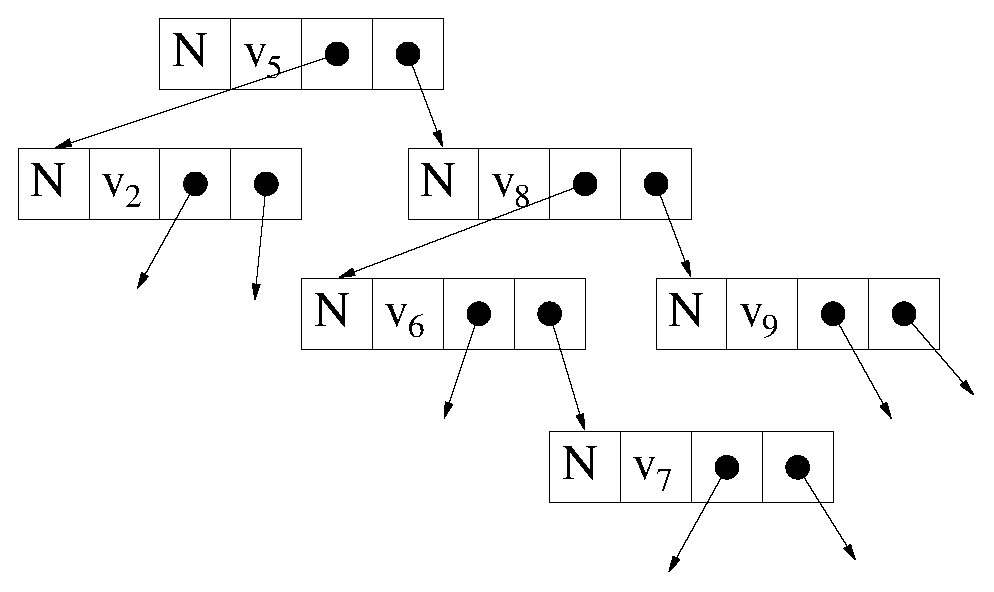
\includegraphics[scale=0.5]{1-Introduction/fig/destructive/data-tree}
\end{center}

For a small number of values, using a binary tree is \emph{worse} than copying the whole array for each update, because each node contains an object header and two pointers instead of just a value. A balanced tree of 1000 elements is 10 levels deep, and as a rough approximation, half of the nodes lie at the bottom of the tree. If we were to update one of these nodes then we would need to reallocate all of its parents, which equates to 9 * 4 = 36 words of space. Not all nodes are at this level, but we haven't accounted for finding the node to be updated in the first place either. For a back-of-envelope calculation we could expect an average of at least 50 machine instructions to be required to update a node in this tree. This equates to 2\% efficiency when compared with destructive array update of a similarly sized array.

Another option is to use trees of a higher order, perhaps a quadtree or a B-tree structure like the one shown in the following diagram. Adding more values per node reduces the depth of the tree. It also reduces the number of nodes we must rebuild when performing an update, but at the cost of making each node larger. 

\begin{center}
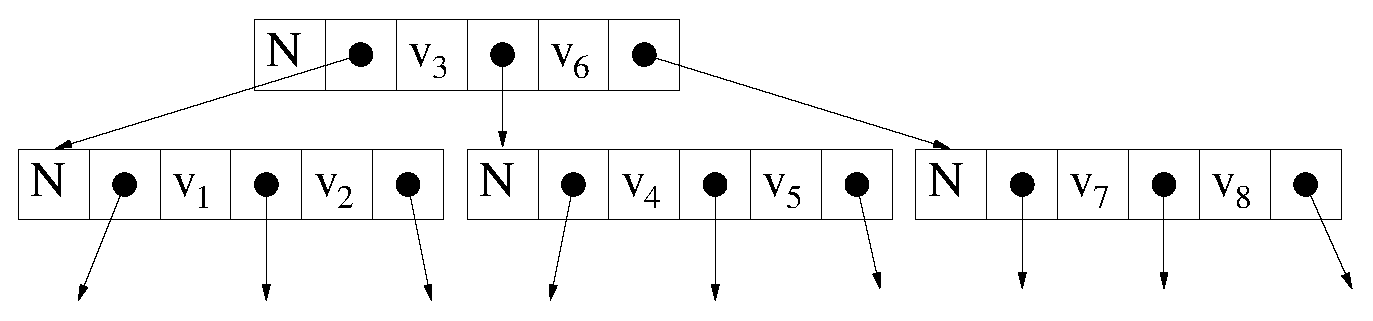
\includegraphics[scale=0.5]{1-Introduction/fig/destructive/data-btree}
\end{center}

For a full (2,3)-tree with two keys and three branches per node, each node is 6 words long including the object header. Every extra level provides three times the number of nodes present in the previous level, and for 1000 values we need a little more than 6 levels. If we say that each node to be updated has an average of 5 parent nodes, this equates to 5 * 6 = 30 words of space to be reinitialised when updating a node. This isn't much better than the previous case.

Many algorithms naturally use an array as their primary collection structure. If, for the lack of destructive update, we are forced to a tree instead, then we automatically impose a $\log(n)$ slowdown on our algorithm's run time. To access an element in a tree we must traverse its structure, but array access can be performed in constant time. This slowdown is in addition to a substantial constant factor due to the extra book-keeping data that must be maintained, such as object headers and branch pointers that are not needed when using arrays. In \cite{ponder:inefficient} Ponder gives a list of algorithms for which no equivalent, array-less algorithm of similar complexity is known. 


% --------------------
\subsubsection{The limit}
There are an infinite variety of possible structures for simulating arrays, and trees represent just a few. By this stage, an astute reader may be thinking about all their own favourite structures and how much better they are than the ones outlined here \cite{okasaki:pure-data, okasaki:intmaps}. As we are talking about machine instructions and constant factors, not just algorithmic complexity, there are also a huge variety of low level details to consider. Details include instruction selection, caching, data layout, pointer compression \cite{lattner:pointer-compression}, and using ``diff arrays'' which rely on destructive update behind the scenes for efficiency, whilst presenting a functionally pure interface. An example of pointer compression is to replace each of the pointers in an object by offsets from a base pointer, instead of including the store address in full. This can result in substantial space savings for pointer heavy programs on 64 bit machines, where the size of a particular data structure is only a tiny fraction of the available address space. Diff arrays use a destructively updateable array for the current state of the structure, and updates to the structure are implemented by physically updating this array. Old states of the array are represented by a list of differences to apply to the current state, so old states become slower and slower to access as the program progresses.

There are many avenues for improvement, but without destructive update we are still hamstrung by the need to allocate objects to represent new program states. Consider a maximally efficient structure which requires only a single, tiny object to be allocated for each update. At the least, we could expect this new object to contain a header word, the new value, and a pointer to the rest of the structure: 

\begin{center}
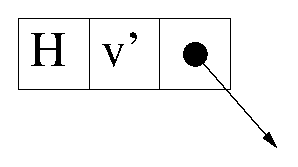
\includegraphics[scale=0.5]{1-Introduction/fig/destructive/data-tiny}
\end{center}

\vspace{-1em}
However, the allocation and initialisation of this object will still require at least five machine instructions, three for allocation and two to write the new value and pointer. For some applications a constant five-fold slow down is of no consequence, but for others it is a deal breaker. 


\clearpage{}
% --------------------
\subsubsection{Tuples and records are also arrays}

At the machine level, tuples and record objects are often very similar to arrays. We can implement records by representing each field as a pointer to the object containing its value, so at this level the record is simply an array of pointers. A record object with 5 fields would contain a header word and five pointers. Consider then the following record type from DDC:

\begin{lstlisting}
data SquidS 
    = SquidS
    { stateTrace           :: Maybe Handle			
    , stateTraceIndent     :: Int
    , stateErrors          :: [Error]
    , stateStop            :: Bool 
    , stateArgs            :: Set Arg	
    , stateSigmaTable      :: Map Var Var
    , stateVsBoundTopLevel :: Set Var
    , stateVarGen          :: Map NameSpace VarBind 
    , stateVarSub          :: Map Var  Var 
    , stateGraph           :: Graph
    , stateDefs            :: Map Var Type
    , statePath            :: [CBind]
    , stateContains        :: Map CBind (Set CBind)
    , stateInstantiates	   :: Map CBind (Set CBind)
    , stateGenSusp         :: Set Var
    , stateGenDone         :: Set Var
    , stateInst            :: Map Var (InstanceInfo Var Type)			
    , stateQuantifiedVars  :: Map Var (Kind, Maybe Type)
    , stateDataFields      :: Map Var ([Var], [(Var, Type)]) 
    , stateProject         :: Map Var (Type, Map Var Var)	
    , stateProjectResolve  :: Map Var Var
    , stateClassInst       :: Map Var [Fetter] }
\end{lstlisting}

This record represents the state of our type inferencer while it is reducing constraints. The meaning of the fields is not important for this discussion. We include this data type to make the point that real records can contain upwards of 22 separate fields. No matter how efficiently the internal sets, maps and graphs are implemented, without destructive update we cannot change the value of a field without rebuilding at least part of the record object. If we must rebuild it all, then this is at least 22 times slower than using destructive update.

In a language without destructive update we must allocate and initialize new objects to represent new program states. This a drastically less efficient alternative. In practice, even if a language does not support the destructive update of arbitrary structures, attempts are made to introduce it in a more restricted form. In \cite{sastry:order-of-evaluation-analysis} Sastry presents an analysis to determine an order of evaluation for array access and update operations, that allows the updates to be implemented destructively. Besides being first order only, the trouble with many such analyses is that when they fail to introduce an update at an important point in the program, the programmer is left with little recourse to add it manually. There is also the problem of determining which updates \emph{should} have been implemented destructively, but weren't. 

As discussed in \S\ref{intro:monads}, Haskell includes a monadic sub-language that supports the destructive update of select structures such as arrays. However, this sub-language introduces its own problems, and algebraic data such as records and lists cannot be similarly updated. In \cite{sansom:time-profiling} Sansom describes the time profile of an early version of GHC, and mentions that the use of a monadic mutable array over an association list improved the performance of type substitution by a factor of 10. When combined with other improvements, this resulted in a 20x speedup of the type checker as a whole.
 
If a particular programmer does not use functional arrays or large records in their programs, then they may not be aware of the run-time cost of using them. However, those who do are looking down the barrel of a five fold slow-down, or worse, compared with other languages.


% --------------------
\subsection{Destructive update helps to broadcast new values}
\label{Intro:Update:broadcast}
There is an often rehearsed argument that the expressiveness of a language is more important than efficiency, because improvements to processor speed will quickly recover any lost ground. The standard counter is to say that the common man wants their new and faster computers to do \emph{new and faster things}, not the original things less efficiently.

These arguments can also be applied to destructive update. ``Surely'', the antagonist offers, ``a five fold slow-down is not \emph{that} bad. Moore's law says we'll have that back in four years, and look at all the extra compiler optimisations we can do now that the language is pure!''.

Computational efficiency may or may not matter to a particular programmer, but the level of abstraction offered by the language should matter to all. We will now move away from concerns over run time speed, and instead focus on the expressiveness of the language itself. Consider a set of program modules which all reference a single, shared value. This value could be a cursor position or timing value, something that changes often and is of interest to many separate modules. We will refer to this value as X. In a language with destructive update we can place X in a container structure and have each module access it via a pointer:

\begin{center}
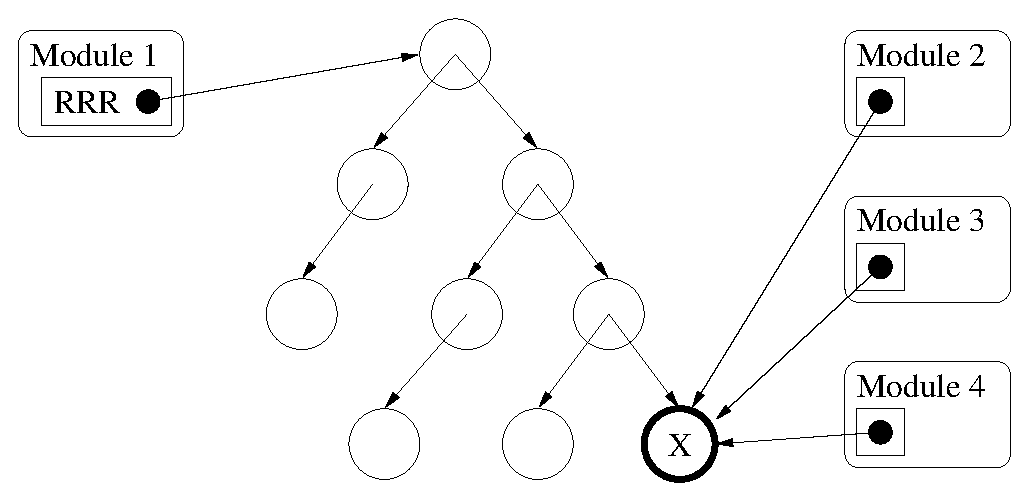
\includegraphics[scale=0.6]{1-Introduction/fig/destructive/broadcast-direct}
\end{center}

Using destructive update, one module can modify X and the new version is immediately visible to others. Notice that module 1 has a reference to the top of the container structure as well as a description of how to find the value of interest. In this example the container is a binary tree and the value is accessable by following three right branches from the root node. On the other side, modules 2, 3, and 4 do not need to know how to locate X within its container because they have a pointer directly to it. This second group of modules is not interested in the container or any other value contained within.

Without destructive update, a module cannot change X directly, nor can it change the pointers within client modules so that they reference any new objects it might create. The programmer is forced to rewrite all modules so that they reference the top level of the container structure, and include a description of how to find the value of interest.

\begin{center}
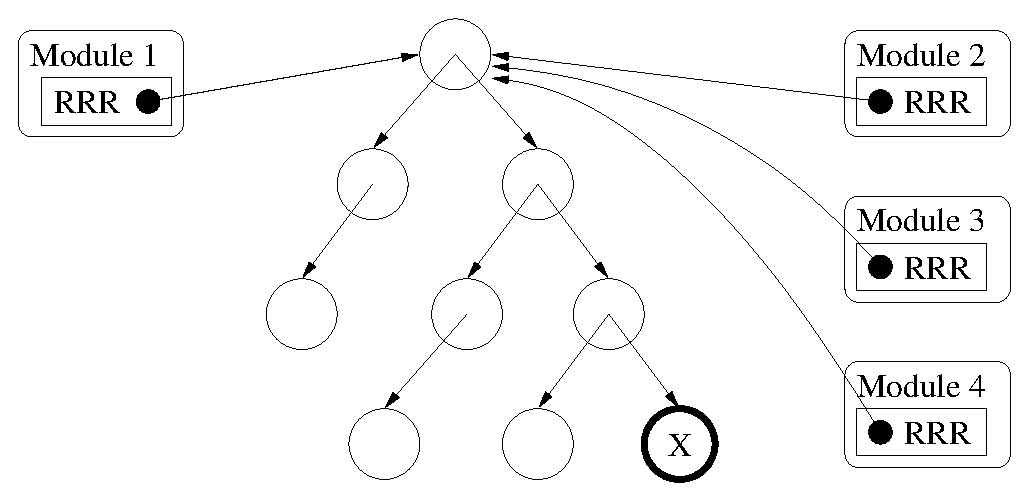
\includegraphics[scale=0.6]{1-Introduction/fig/destructive/broadcast-toplevel}
\end{center}

By doing this we have reduced the level of abstraction in the program. Whereas modules 2, 3, and 4 are only interested in the value X, they must now also concern themselves with the container structure and how to find and update elements contained within.

This problem is compounded when a shared value is logically part of several containers. Perhaps X is also present in a graph structure, and the tree is used to represent a set of objects which must be written to disk when the program finishes. The modules that wish to update the shared value must have knowledge of all structures which contain it.

Shared values like the one described here are often needed to write interactive programs such as Frag \cite{cheong:frag}. In Haskell, variables holding timing values, mouse positions and other user interface states are typically bundled up into a record of IORefs. This in turn requires all code which accesses these values to be written in the IO monad, a point we will return to in \S\ref{intro:monads}.


% --------------------
\subsubsection{Updating nested records in Haskell is painful}

Haskell 98 has an conspicuously poor record system. In itself this is not a new observation, but we pause to discuss it because we feel the problem arises in part from the lack of destructive update in the ambient language. Standard complaints include the records not being light weight, not being extensible, and that all field names are in the top level scope \cite{peyton-jones:records}. In addition, we consider the syntax for updating nested records to be unusable.
 
The following code defines three record types with two fields each. Type \texttt{R1} contains type \texttt{R2}, and type \texttt{R2} contains type \texttt{R3}. Notice the prefixes \texttt{r1}, \texttt{r2} and \texttt{r3} on each field name. In Haskell, field names pollute the top level name space, so we can't have a field named \texttt{field1} in \texttt{R1} as well as in \texttt{R2} without creating a name clash.

\clearpage{}
\begin{lstlisting}
data R1 = R1 { r1Field1  :: Int
             , r1Field2  :: R2 }

data R2 = R2 { r2Field1  :: Char
             , r2Field2  :: R3 }

data R3 = R3 { r3Field1  :: Bool
             , r3Count   :: Int }
\end{lstlisting}

We will create a record value of type \texttt{R1} as an example. Similarly to the previous section, we treat the field \texttt{r3Count} as a shared value that many program modules will be interested in. When the record is created we will initialise this field to zero. The exact values used for the other fields are not important for this example.

\begin{lstlisting}
record1 = R1 { r1Field1 = 5
             , r1Field2 = 
                  R2 { r2Field1 = 'a'
                     , r2Field2 =
                          R3 { r3Field1 = False
                             , r3Count  = 0 }}}
\end{lstlisting}

Extracting the counter field from the structure is straightforward. Each field name becomes a projection function which takes the record and produces the field value, for example \texttt{r1Field1 :: R1 -> Int}. We can make use of the function composition operator to extract the count field using a pleasing syntax:

\begin{lstlisting}
count  = (r3Count . r2Field2 . r1Field2) record1
\end{lstlisting}

Updating the counter is another matter entirely. As we do not wish to modify the other fields in the structure, we must unpack and repack each level in turn. This process corresponds to reallocating parents when updating a node in a tree. Unfortunately, this time we cannot write a cute recursive function to do so because the records at each level have different types. The following diagram shows the structure of the nested records:

\begin{center}
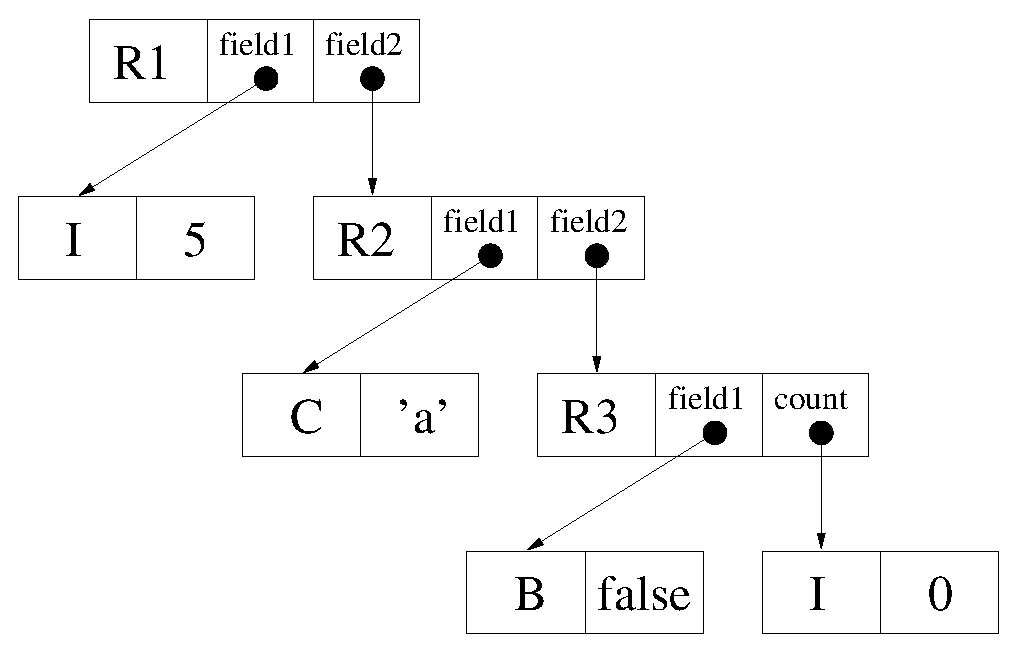
\includegraphics[scale=0.5]{1-Introduction/fig/destructive/broadcast-record}
\end{center}

\clearpage{}
\begin{center}
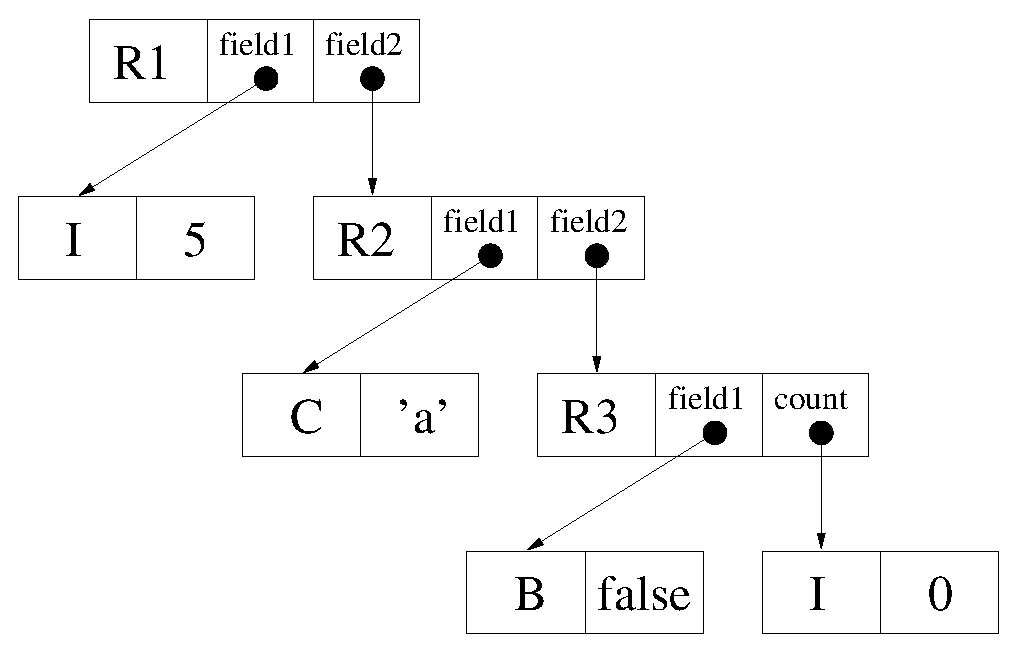
\includegraphics[scale=0.5]{1-Introduction/fig/destructive/broadcast-record}
\end{center}

If we wish to change the \emph{count} field in this structure to the value 1, we must allocate a new object containing this value. We must then rebuild the \texttt{R3}, \texttt{R2} and \texttt{R1} nodes so that the structure references this new object while retaining the pointers to the other nodes. Here is the gory Haskell expression:

\begin{lstlisting}
record2
  = record1 { r1Field2 = 
      (r1Field2 record1) { r2Field2 = 
         ((r2Field2 . r1Field2) record1) { r3Count = 1 }}}
\end{lstlisting}

Clearly this is not something a typical programmer would enjoy writing. The field names and the variable \texttt{record1} are repeated twice each, the line must be broken into fragments to fit on the page, it does not indent well, and there is much visual noise.

It is worse when we need to update this field with a non-trivial expression. Consider the simple act of incrementing \texttt{r3Count}. We can use layout to reduce the noise, but it is still quite bad:
\begin{lstlisting}
record3
  = record2 { 
      r1Field2 = (r1Field2 record2) {
      r2Field2 = ((r2Field2 . r1Field2) record2) {
      r3Count  = (r3Count . r2Field2 . r1Field2) record2 + 1 
    }}}
\end{lstlisting}
The need to write such tedious code to perform such a simple update would be a deal breaker for many programmers.\footnote{It certainly is for the author.}

Consider an equivalent statement in an imperative language, such as C++.
\begin{lstlisting}
record2.field2.field2.count += 1
\end{lstlisting}
Destructive update allows the programmer to focus solely on the element of interest, while leaving the others untouched. Granted, the above statement does not have the same semantics as the Haskell version because it modifies the original object instead creating a new one. If this behaviour is required then many imperative, object oriented languages support a fragment such as:
\begin{lstlisting}
record3 = record2.copy()
record3.field2.field2.count += 1
\end{lstlisting}
To the surrounding program these two simple statements have the same effect as the Haskell expression shown above, with the added advantage that the concepts of \emph{copy} and \emph{update} are clearly separated.

In C++ we can make life even easier for the programmer. We can create a reference to the field of interest and increment it without any knowledge of the surrounding record structure:
\begin{lstlisting}
int* countRef = &(record.field2.field2.count)

(*countRef) += 1;
\end{lstlisting}

Admittedly, references and destructive update can be used for evil as well as for good. Many confusing programs can be constructed in which different program modules communicate via shared mutable objects in a way which is entirely non-obvious to the casual observer, and almost impossible to debug. The counter to this argument is to say that confusing programs can be written in any language, and a good carpenter can hammer a nail into a wall without smashing their own fingers.

We should note that the problem of updating nested records in Haskell can be made easier by generic programming libraries such as `Scrap Your Boilerplate'~\cite{lammel:scrap-your-boilerplate} (SYB) and DriFT~\cite{hinze:generic-programming-in-haskell}. Although these systems can help, we feel they are not complete solutions as they lack the efficiency and ease of use of destructive update. SYB style systems tend to traverse uninteresting parts of a structure when performing an update, resulting in a significant performance penalty~\cite{mitchell:neil}. DriFT is a preprocessor which can automatically generate update functions for each of the fields in a record, though it does not support nested update as per the previous example. When implementing DDC we defined tuples of get and set functions for each field, along with combinators to compose these functions and to update fields deep within nested records. We have found this to be a serviceable yet tedious approach, as we have not yet written a preprocessor to generate the tuples. This approach also does not solve the problem of field names being in top level scope.


\clearpage{}
\section{Constraints and evidence}
\label{Core:Witnesses}

% ---------------------------------------------------------
\subsection{Witness passing}
\label{Core:Witnesses:evidence}
Consider the Haskell function $\ipairEq$ which tests if the two elements of a pair are equal:

\code{
	$\ipairEq :: \forall a. \ \iEq \ a \Rightarrow (a, \ a) \rightarrow \iBool$ \\
	$\ipairEq \ (x, \ y) \ = \ x == y$
}

In the type signature, the constraint $\iEq \ a$ restricts the types that $a$ can be instantiated with to just those which support equality. This requirement arises because we have used $(==)$ to compare two values of type $a$.

As well as being a type constraint, a Haskell compiler such as GHC would treat $\iEq \ a$ as the type of an extra parameter to $\ipairEq$. In this case, the parameter will include an appropriate function to compare the two elements of the pair. During compilation, the compiler will detect applications of $\ipairEq$ and add an extra argument appropriate to the type it is called at. For example, a GHC style translation of $\ipairEq$ to its core language \cite{hall:type-classes} would yield something similar to:

\code{
	\mc{2}{$\ipairEq$} \\
	\ = 	& $\Lambda \ a$		& $: *.$ \\
		& $\lambda \ \icomp$	& $: (a \to a \to \iBool).$ \\
		& $\lambda \ \ipair$	& $: (a, \ a).$ \\
		& \mc{2}{$\kcase \ \ipair \ \kof$} \\
}

\vspace{-3ex}
\code{		
	& & \quad $(x, \ y) \to \icomp \ x \ y$
}

while an application of this function in the source language:

\code{
	$\ipairEq \ (2, 3)$
}

would be translated to:

\code{
	$\ipairEq \ \iInt \ \iprimIntEq \ (\iPair \ \iInt \ 2 \ 3)$
}

where $\iprimIntEq$ is the primitive equality function on integers. 

Returning to the translation of $\ipairEq$, the extra parameter $\icomp$ binds \emph{evidence} \cite{jones:qualified-types} that type $a$ really does support the equality operation -- and there is no better evidence than the function which performs it. 

With this in mind, suppose that we were only interested in the fact that $\ipairEq$ requires $a$ to support equality, rather than how to actually evaluate this function at runtime. In the above translation, we managed our evidence at the value level, by explicitly passing around a comparison function. Alternatively, we could manage it at the type level:

\code{
	\mc{2}{$\ipairEq$} \\
	\ = 	& $\Lambda \ a$		& $: *.$ \\
		& $\Lambda \ w$		& $:\iEq \ a.$ \\ 
		& $\lambda \ \ipair$	& $: (a, \ a).$ \\
		& \mc{2}{$\kcase \ \ipair \ \kof$} \\
}

\vspace{-3ex}
\code{
	& & \quad $(x, \ y) \rightarrow (==) \ w \ x \ y$
}


\medskip
In this new translation the extra parameter, $w$, binds a \emph{proof term}. One step removed from value-level evidence, this type-level proof term serves as \emph{witness} that type $a$ really does support equality, and this is recorded in its kind $\iEq \ a$. Now, the application of $(==)$ to the elements of the pair requires type $a$ to support equality, and we satisfy this requirement by passing it our witness to the fact. 

How a particular calling function happens to manufacture its witnesses is of no concern to $\ipairEq$, though they do need to enter the system somehow. In the general case, a caller has three options: require the witness to be passed in by an outer function, combine two witnesses into a third, or construct one explicitly.

For this example, the third option suffices, and we can translate the call as:

\code{
	$\ipairEq \ \iInt \ (\iMkEq \ \iInt) \ (\iPair \ \iInt \ 2 \ 3)$
}

The type level function $\iMkEq$ is a \emph{witness constructor} which takes a type, and constructs a witness of kind $Eq \ a$. The expression $(\iMkEq \ \iInt)$ is as an axiom in our proof system, and it is valid to repeat it in the program when required. In contrast, when we discuss witnesses of constancy and mutability in \S\ref{Core:Witnesses:mutability}, their construction will be restricted to certain places in the program, to ensure soundness.

With this plumbing in place we can ensure our code is consistent with respect to which types support equality (or mutability), simply by type checking it in the usual way and then inspecting the way witnesses are constructed.


% ---------------------------------------------------------
\subsection{Dependent kinds}

Dependent kinds are kinds that contain types, and in DDC we use them to describe witness constructors. Dependent kinds were  introduced by the Edinburgh Logical Framework (LF) \cite{avron:edinburgh-lf} which uses them to encode logical rules, and aspects of this framework are present in our core language. Types are viewed as assertions about values, and kinds are viewed as assertions about types. 

Functions that take types to kinds are expressed with the $\Pi$ binder, and we apply such a function by substituting its argument for the bound variable, as usual. For example:

$$	\frac
		{ \emptyset \judge \iMkEq :: \Pi(a : *). \ \iEq \ a 
	  	\qq
	  	\emptyset \judge \iInt :: *
		}
		{ \emptyset \judge \iMkEq \ \iInt :: \iEq \ \iInt }
$$

Note that $\iMkEq \ \iInt$ is a type term, and $\iEq \ \iInt$ is a kind term. In this chapter we use the convention that type constructors starting with ``$\iMk$'' produce witnesses.


% ---------------------------------------------------------
\subsection{Witnesses of mutability}
\label{Core:Witnesses:mutability}
When optimising programs involving destructive update, it is of crucial importance that we do not lose track of which regions are mutable and which are supposed to be constant. As mentioned earlier, DDC uses the witness passing mechanism to keep track of this information, both to guide optimisations and as a sanity check on the intermediate code.

Of primary concern are functions that destructively update objects in the store. For example, ignoring effect and closure information, the $\iupdateInt$ function from \S\ref{System:Effect:information-in-types} has type:

\code{
	$\iupdateInt$
		$:: \forall r_1 \ r_2. \
		\iMutable \ r_1 \Rightarrow 
		\iInt \ r_1 \rightarrow \iInt \ r_2 \rightarrow ()$
}

Using ideas from \S\ref{Core:Witnesses:evidence}, we treat the region constraint \mbox{$Mutable \ r_1$} as the kind of an extra type parameter to this function. As we are now considering such constraints to also be type \emph{parameters}, we write them in prefix form with $\Rightarrow$ instead of in postfix form with $\rhd$ as we did in the source language.

When we call $\iupdateInt$ we must pass a witness to the fact that $r_1$ is indeed mutable, and we now consider how these witnesses should be constructed. We could perhaps construct them directly at call-sites as per our $\ipairEq$ example. However, unlike the type class situation, the various region class witnesses are not necessarily compatible. For example, there is nothing wrong with  $\iMkEq \ a$ and $\iMkShow \ a$ existing in the same program, but if we have both $\iMkMutable \ r_1$ and $\iMkConst \ r_1$ then something has gone badly wrong.

If we were to allow region witnesses to be constructed anywhere in the intermediate code, then the compiler would need access to the whole program to ensure that multiple incompatible witnesses are not constructed for the same region. This would be impossible to implement with respect to separate compilation.

Instead, we require that all witnesses involving a particular region variable are constructed at the same place in the code, namely the point where the variable itself is introduced. As in \cite{tofte:mlkit-4.3.0}, we use $\kletregion$ to bring region variables into scope. Here is an example program which creates and integer, updates it, and then prints it to the console:

\code{
	$\iprintMe :: \ () \to ()$ \\
}

\vspace{-3ex}
\code{	\mc{3}{$\iprintMe$} \\
	\ $=$	& $\lambda ().$ \\
		& $\kletregion \ r_1 \ \kwith \ \{ \ w_1 = \iMkMutable \ r_1 \ \}$	& $\kin$ \\
		& $\kletregion \ r_2 \ \kwith \ \{ \ w_2 = \iMkConst \ r_2 \ \}$	& $\kin$ \\
}

\vspace{-3ex}
\code{
		& & $\kdo$ \\
		& & & $x$		& $= \ 5 \ r_1$ \\
		& & & \mc{2}{$\iupdateInt \ r_1 \ r_2 \ w_1 \ x \ (23 \ r_2)$} \\
		& & & \mc{2}{$\iprintInt \ r_1 \ x$}
}

Note that in the core language, literal values such as `$5$' act as constructors that take a region variable and allocate a new object. This gives $x$ the type $\iInt \ r_1$. The only place the constructors $\iMkMutable$ and $\iMkConst$ may be used is in the set of witness bindings associated with a $\kletregion$. In addition, we may only create witnesses for the region variable being introduced, and we cannot create witnesses for mutability and constancy in the same set. This ensures that conflicting region witnesses cannot be created.

To call the $\iupdateInt$ function we \emph{must} have a witness that $r_1$ is mutable. Trying to pass another witness, like the one bound to $w_2$, would result in a type error. With this encoding, it is easy to write code transformations that depend on whether a particular region is mutable or constant. Such a transformation can simply collect the set of region witnesses that are in scope while descending into the abstract syntax tree. We will see an example of this in \S\ref{Core:Optimisation:full-laziness}.


% --------------------
\subsection{Witnesses of purity}
\label{Core:Witnesses:purity}
When translating a program which uses lazy evaluation to the core language, we must also construct witnesses of purity. Recall from \S\ref{System:Effects:purification} that the type of $\isuspend$ is:

\code{
 	$\isuspend$ & 
	$:: \forall a \ b \ e_1. \ \iPure \ e_1 \Rightarrow (a \lfuna{e_1} b) \to a \to b$ \\
}

$\isuspend$ takes a function of type $a \funa{e_1} b$, its argument of type $a$ and builds a thunk that represents the suspended function application. When the thunk is forced, the function will be applied to its argument yielding a result of type $b$. The $\iPure \ e_1$ constraint ensures that the function application being suspended has no visible side effects, so the value of its result will not depend on when it is forced.

We now consider how witnesses of purity are created in the core language. Consider the following source program:

\code{
	$\ifun$
		& $::$		& $\forall a \ r_1\ r_2 \ e_1$ \\
		& $.$		& $(\iInt \ r_1 \lfuna{e_1} a) \to \iBool \ r_2 \to a$ \\
		& $\rhd$	& $\iPure \ e_1, \ \iConst \ r_2$
}

\code{
	\mc{3}{$\ifun \ f \ b$} \\
	\ $=$	& $\kdo$	& $g \ x$	& $= \kif \ x \ \kthen \ f \ 5 \ \kelse \ f \ 23$ \\
		&		& \mc{2}{$\isuspend \ g \ b$}
}

$\ifun$ causes its first parameter to be applied to either 5 or 23, depending on whether its second is true or false. This is done by an auxiliary function, $g$, and the application of this function is suspended. Because the application of $g$ is suspended it must be pure. Note that the purity of $g$ relies on two separate facts: that $f$ is pure, and that $x$ is constant. 

Here is $\ifun$ converted to the core language:

\hspace{-3em}
\code{
	\mc{3}{$\ifun$} \\
	\ $=$	& \mc{2}{$\Lambda \ a \ r_1 \ r_2 \ e_1.$} \\
		& $\Lambda \ (w_1$	& $: \iPure \ e_1).$ \\
		& $\Lambda \ (w_2$	& $: \iConst \ r_2).$ \\
		& $\lambda \ (f$	& $: \iInt \ r_1 \lfuna{e_1} a).$ \\
		& $\lambda \ (b$	& $: \iBool \ r_2).$ 
}	

\vspace{-3ex}
\hspace{-3em}
\code{
	& & $\kdo$ \\
	& & & $g$	& \mc{2}{$= \lambda (x : \iBool \ r_2). 
						\ \kif \ x \ \kthen \ f \ (5 \ r_1) \ \kelse \ f \ (23 \ r_1)$} 
}

\vspace{-2ex}
\hspace{-3em}
\code{	
	& & & & $\isuspend$	& $(\iMkPureJoin \ e_1 \ (\iRead r_2) \ w_1 \ (\iMkPurify \ r_2 \ w_2)$) \\
	& & & &			& $g \ b$
}

When we call $\isuspend$, the term $(\iMkPureJoin \ e_1 \ (\iRead r_2) \ w_1 \ (\iMkPurify \ r_2 \ w_2))$ builds a witness to the fact that $g$ is pure. Note that in this chapter we treat $\isuspend$ as a primitive, so we do not need applications for the argument and return types, or the effect of the function. The typing rule for $\isuspend$ takes care of this parameterisation.

The witness to the purity of $g$ is constructed from two simpler witnesses, one showing that $e_1$ is pure, and another showing that the read from $r_2$ is pure. The first is given to us by the calling function, and is bound to $w_1$. 

The second is constructed with the $\iMkPurify$ witness constructor which has kind:

\code{
	$\iMkPurify :: \Pi(r : \%). \iConst \ r \to \iPure \ (\iRead \ r)$
}

This kind encodes the rule that if a region is constant, then any reads from it can be considered to be pure. When we apply $\iMkPurify$ to $r_2$, this variable is substituted for both occurrences of $r$ yielding:

\code{
	$(\iMkPurify \ r_2) :: \iConst \ r_2 \to \iPure \ (\iRead \ r_2)$
}

From the $\Lambda$-binding at the beginning of the function we have $w_2 :: \iConst \ r_2$, so applying $w_2$ as the final argument gives:

\code{
	$(\iMkPurify \ r_2 \ w_2) :: \iPure \ (\iRead \ r_2)$
}

Which shows that a read from $r_2$ is indeed pure.

What remains is to join the two simple witnesses together. This is done with the $\iMkPureJoin$ witness constructor which has kind:

\code{
	\mc{3}{$\iMkPureJoin$}	\\
	& $::$	& $\Pi(e_1 :: \ !). \ \Pi(e_2 :: \ !)$ \\
	& $.$	& $\iPure \ e_1 \to \iPure \ e_2 \to \iPure \ (e_1 \lor e_2)$
}

Applying the first two arguments gives:

\code{
	\mc{3}{$(\iMkPureJoin \ e_1 \ (\iRead \ r_2))$} \\
	& $::$	& $\iPure \ e_1 \to \iPure \ (\iRead \ r_2) \to \iPure \ (e_1 \lor \iRead \ r_2)$
}

This says that if we have a witness that the effect $e_1$ is pure and a witness that the effect $\iRead \ r_2$ is pure, the combination of these two effects is also pure. Our final witness then becomes:

\code{
	\mc{3}{$(\iMkPureJoin \ e_1 \ (\iRead \ r_2) \ w_1 \ (\iMkPurify \ r_2 \ w_2))$} \\
	& $::$	& $\iPure \ (e_1 \lor \iRead \ r_2)$
}

The effect $e_1 \lor \iRead \ r_2$ is exactly the effect of $g$, so the above witness is sufficient to prove that we can safely suspend a call to it.

Note that we do not need witnesses of \emph{impurity}. The fact that an expression is pure gives us the capability to suspend its evaluation, and by constructing a witness of purity we prove that this capability exists. In contrast, the fact that an expression is impure is not a capability, because it does not allow us to do anything ``extra'' with that expression.











%!TEX root = ../Main.tex

\begin{figure}
\boxfig{
\begin{tabbing}
MMM              \= MM   \= MMMMMMMMMMMMMMMMM   \= MMM \= MM \= MMMMMMMM    \kill
\textbf{Indices} \> \>                 \> \textbf{Names} \\
$ix$ \> $\to$   \> (debruijn index)    \> $a,~ r,~ e$ \> $\to$ \> (type variables)     \\
$p$  \> $\to$   \> (region identifier) \> $z$         \> $\to$ \> (term variables)     \\
$l$  \> $\to$   \> (store location)
\\
\\

\textbf{Kinds} ($k$)\\
$\mkind$
        \> ::=   \> $\kcData ~~|~~ \kcRegion ~~|~~ \kcEffect$
        \> (kind constructors)
\\
        \> $~|~$ \> $\mkind \kto \mkind$ 
        \> (function kind)
\\
\\


\textbf{Types} ($t,~ r,~ e$)\\
$\mtype$  
        \> ::=  \> $ix\bra{a}$
        \> (debruijn index\bra{variable})
\\
        \> $~|~$  \> $\forall \bra{a} : \mkind.~~ \mtype$
                        $~|~$ $\mtype~~ \mtype$
        \> (universal quantifier, type application)
\\
        \> $~|~$  \> $\mtype ~+~ \mtype$
                        $~|~$ $\bot$           
        \> (effect join and bottom) 
\\        
        \> $~|~$  \> $\mtycon_n$        
        \> (type constructor)
\\      
        \> $~|$   \> $\trgn{p}$
        \> (region handle)
\\
\\


\textbf{Type Constructors} ($\mtc$)\\
$\mtycon_0$ 
        \> ::=  \> $(\to)
                        ~~|~~ \tcUnit
                        ~~|~~ \tcBool
                        ~~|~~ \tcNat$
\\
$\mtycon_1$ 
        \> ::=  \> $\tcRead
                        ~~|~~ \tcWrite
                        ~~|~~ \tcAlloc$
\\
$\mtycon_2$ 
        \> ::=  \> $\tcRef$
\\ 
\\


\textbf{Values} ($v$)\\
$\mval$ \> ::=  \> $ix\bra{z} ~~|~~ \mconst$ 
        \> (debruijn index\bra{variable}, constant)
\\
        \> $~|$ \> $ \lambda \bra{z} : \mtype.~ \mexp
               ~~|~~ \Lambda \bra{a} : \mkind.~ \mexp$
        \> (value and type abstraction)
\\
        \> $~|$ \> $\vloc{l}$
        \> (store location)
\\
\\


\textbf{Expressions} ($x$)\\
$\mexp$ \> ::=  \> $\mval
                        ~~|~~ \mval~~ \mval
                        ~~|~~ \mval~~ \mtype$
        \> (value, value and type application)
\\
        \> $~|$ \> $\xlet{\bra{z}}{\mtype}{\mexp}{\mexp}$
        \> (let-binding)
\\
        \> $~|$ \> $\mop_n~ \ov{\mval}^{\; n}$
        \> (fully applied pure operator)
\\
        \> $~|$ \> $\xprivate{\bra{r}}{\mexp}$
        \> (define a private region)
\\
        \> $~|$ \> $\xextend{\mtype}{\bra{r}}{\mexp}$
        \> (extend an existing region)
\\
        \> $~|$ \> $\kalloc~~ \mtype~~ \mval$
        \> (allocate a store binding)
\\
        \> $~|$ \> $\kread~~~~  \mtype~~ \mval$
        \> (read a store binding)
\\
        \> $~|$ \> $\kwrite~~ \mtype~~ \mval~~ \mval$
        \> (write a store binding)
\\
\\


\textbf{Constants} ($c$)\\
$const$ \> ::=  
        \> $\tt{unit} 
                ~|~ \tt{tt}
                ~|~ \tt{ff}
                ~|~ \tt{0} 
                ~|~ \tt{1} 
                ~|~ \tt{2}
                ~|~ ...$
        \> (data constants)
\\
\\

\textbf{Pure Operators} ($o$)\\
$\mop_1$
        \> ::=  \> $\tt{isZero} 
                        ~~|~~ \tt{succ}$
        \> (pure operators)
\end{tabbing}
} % boxfig
\medskip
\caption{\SystemFre grammar.}
\label{f:Language}
\end{figure}

\section{Comparisons}

\subsection{Monadic intermediate languages. 1998 --\\
	 Tolmach, Benton, Kennedy, Russell.}
\label{Core:Comparisons:monadic-intermediate-languages}
One of the main inspirations for our work has been to build on the monadic intermediate languages of \cite{tolmach:optimizing-ml}, \cite{benton:monads-effects-transformations} and \cite{peyton-jones:bridging-the-gulf}. The system of \cite{tolmach:optimizing-ml} uses a coarse grained effect analysis to guide the translation of the source program into a core language incorporating a hierarchy of monadic types. The monads are \texttt{ID}, \texttt{LIFT}, \texttt{EXN}, and \texttt{ST}. Starting from the bottom of the hierarchy: \texttt{ID} describes pure, terminating computations; \texttt{LIFT} encapsulates pure but potentially non-terminating computations; \texttt{EXN} encapsulates potentially non-terminating computations that may raise uncaught exceptions, and \texttt{ST} encapsulates computations that may do everything including talk to the outside world.

The optimisations in \cite{tolmach:optimizing-ml} are given as transform rules on monadic terms, and less transforms apply to expressions written with the more effectual monads. Limitations of this system include the fact that it lacks effect polymorphism, and the coarseness of the hierarchy. In the last part of \cite{tolmach:optimizing-ml}, Tolmach suggests that it would be natural to extend his system with Hindley-Milner style polymorphism for both types and monads in the Talpin-Jouvelot style. He also suggests that it would extend naturally to a collection of fine-grained monads encapsulating primitive effects, but laments the lack of a generic mechanism for combining such monads. 

\subsubsection{Monads and effects express equivalent information}
In \cite{wadler:marriage-2003}, Wadler and Thiemann compare the effect typing and monadic systems, and give a translation from the first to the second. For their monadic system, they write the types of computations as $\trm{T}^\sigma \ a$, where $a$ is the type of the resulting value and $\sigma$ is a set of store effects. They consider store effects such as $\iRead \ r_1$ and $\iWrite \ r_2$, use $\lor$ to collect atomic effect terms, and include type schemes that quantify over type, region and effect variables. Clearly, their monadic system shares a lot of common ground with an effect system. The main technical difference between the two is that the monadic version of the typing rule for applications is broken into two parts:

Whereas in the effect system we have:

\ruleBox{
	\begin{gather}
	\ruleI	{EffApp}
		{ 	\Gamma \judge t_1 :: \tau_{11} \lfuna{\sigma_3} \tau_{12} \ ; \ \sigma_1
		  \quad \Gamma \judge t_2 :: \tau_{11} \ ; \ \sigma_2 }
		{	\Gamma \judge t_1 \ t_2 :: \tau_{12} \ ; \ \sigma_1 \lor \sigma_2 \lor \sigma_3 }
	\end{gather}
}

In the monadic system we have:

\ruleBox{
	\begin{gather}
	\ruleI	{MonApp}
		{	\Gamma \judge t_1 :: \tau_{11} \to \tau_{12}
		 \quad	\Gamma \judge t_2 :: \tau_{11} }
		{	\Gamma \judge t_1 \ t_2 :: \tau_{12} }
	\ruleSkip
	\ruleI	{MonBind}
		{	\Gamma \judge t_1 : \trm{T}^{\sigma_1} \ \tau_1
		  \quad	\Gamma, \ x : \tau_1 
				\judge t_2 : \trm{T}^{\sigma_2} \ \tau_2 }
		{ 	\Gamma \judge \ \klet \ x \gets t_1 \ \kin \ t_2 :: \trm{T}^{\sigma_1 \lor \sigma_2} \ \tau_2 }
	\end{gather}
}

In the effect typing system, effects are caused by the application of functions, as well as by the evaluation of primitive operators such as $\ireadRef$ and $\iwriteRef$.  In the monadic system, all effects are invoked explicitly with the $\klet \ x \gets t_1 \ \kin \ t_2$ form, which evaluates the computation $t_1$, and then substitutes the resulting value into $t_2$. Function application of the form $t_1 \ t_2$ is always pure.

\subsubsection{Expressing T-monads in Disciple}
Note that $\trm{T}^\sigma \ a$ style computation types are straightforward to express in Disciple, because we can define data types that have effect parameters. For example, eliding region and closure information we can write:

\code{
	$\kdata \ T \ e_1 \ a = \iMkT \ (() \lfuna{e_1} a)$
}

Our $T \ e_1 \ a$ data type simply encapsulates a function that produces a value of type $a$ when applied to the unit value (), while having an effect $e_1$. The monadic return and bind operators are defined as follows:

\code{
	$\ireturnT$	
	& $::$	& $\forall a. \ a \to T \ \bot \ a$ 
	\\[1ex]
	\mc{3}{$\ireturnT \ x \ = \iMkT \ (\lambda (). \  x)$}
}

\code{
	$\ibindT$ \ \ \	
	& $::$		& $\forall a \ b \ e_1 \ e_2$ \\
	& $.$		& $T \ e_1 \ a \to (a \to T \ e_2 \ b) \to T \ e_3 \ b$ \\
	& $\rhd$	& $e_3 = e_1 \lor e_2$
}

\vspace{-1ex}
\code{
	\mc{3}{$\ibindT \ (\iMkT \ f_1) \ \imf_2$} \\
	& \mc{2}{$= \iMkT \ (\lambda (). \ \kcase \ \imf_2 \ (f_1 \ ()) \ \kof$} \\
	& & \qq \qq \qq $\iMkT \ f_2 \to f_2 \ ())$
}

Although we can directly express T monads in a language with an effect system, the reverse is not true. A monadic system requires all effects to be encapsulated within a computation type such as T, and the function arrow, $\to$, must be pure. However, an effect system allows arbitrary function applications to have effects, and we can add these effects as annotations to the arrows, $\funa{\sigma}$.


\subsubsection{What's more natural?}
In \cite{benton:monads-effects-transformations} Benton and Kennedy suggest that ``the monadic style takes the distinction between computations and values more seriously'', and that it has a more well-behaved equational theory. However, their work has different goals to ours. On one hand, \cite{benton:monads-effects-transformations} includes rigorous proofs that their optimising transforms are correct. For this purpose, we can appreciate how reducing effect invocation to a single place in the language would make it easier to reason about. Their system was implemented in the MLj \cite{benton:mlj}  compiler, so it is demonstrably practical. In \cite{benton:relational-semantics-effect-transformations} Benton \emph{et al} consider the semantics of a similar system extended with region variables and effect masking, and in \cite{benton:semantics-effect-analysis} Benton and Buchlovsky present the semantics of an effect based analysis for exceptions. On the other hand, \cite{benton:mlj} does not include effect polymorphism, and the more recent work of \cite{benton:relational-semantics-effect-transformations} and \cite{benton:semantics-effect-analysis} does not discuss type inference and has not yet been implemented in a compiler.  

For our purposes, we find it more natural to think of function application and primitive operators as causing effects, as this is closer to the operational reality. After spending time writing a compiler for a language that includes laziness, we don't feel too strongly about the distinction between computations and values. When we sleep we dream about thunks, and the fact that the inspection of a lazy ``value'' of type $\iInt$ may diverge is precisely because that value represents a possibly suspended computation.  

If we were going to follow Benton and Kennedy's approach then we would write $\trm{T}^{\texttt{LIFT}} \ \iInt$ for the lazy case and $\iInt$ for the direct one. Using (MonBind) above, this would have the benefit that the potential non-termination of lazy computations would be propagated into the types of terms that use them. However, for the reasons discussed in \S\ref{intro:purity} we don't actually treat non-termination as a computational effect. We also remain unconvinced of the utility of introducing a separate monadic binding form into the core language, at least in the concrete implementation. \mbox{Horses for courses.}


\subsection{System-Fc. 2007 -- \\
	Sulzmann, Chakravarty, Peyton Jones, Donnelly.}

The core language of GHC is based on System-Fc \cite{sulzmann:system-Fc}, which uses type equality witnesses to support generalised algebraic data types (GADTs) \cite{xi:grdc} and associated types \cite{chakravarty:associated-types}. The kinds of such witnesses are written $a \sim b$, which express the fact that type $a$ can be taken as being equivalent to type $b$. The witnesses express non-syntactic type equalities, which are a major feature of the work on GADTs and associated types.

 
The witness passing mechanism in DDC was inspired by an earlier draft of \cite{sulzmann:system-Fc} that included the dependent kind abstraction $\Pi a : \kappa_1 . \ \kappa_2$. 

\clearpage{}
In this draft, abstraction was used to write the kinds of polymorphic witness constructors such as:

\code{
	$\ielemList :: \Pi a : *. \iElem \ [a] \sim a$
}

Here, $\iElem$ is the constructor of an associated type. The kind of $\ielemList$ says that elements of a list of type $a$ have type $a$. In the published version of the paper, extra typing rules were introduced to compose and decompose types that include equality constraints, and these new rules subsumed the need for an explicit dependent kind abstraction. In the published version, the type of $\ielemList$ is written:

\code{
	$\ielemList :: (\forall a : *. \iElem \ [a]) \sim (\forall a : *. \ a)$
}

Note that when this type is instantiated, the type argument is substituted for both bound variables. For example:

\code{
	$\ielemList \ \iInt :: \iElem \ [\iInt] \sim \iInt$
}

The dependent kind abstraction is still there in spirit, but the syntax has changed. System-Fc includes witness constructors such as $\isym$, $\itrans$, $\ileft$ and $\iright$ whose kinds express logical properties such as the symmetry and transitivity of the type equality relation, as well as providing decomposition rules. Although \cite{sulzmann:system-Fc} gives typing rules for these constructors, if we were prepared to limit their applicability to first order kinds then we could also express them with the dependent kind abstraction. For example:

\ruleBox{
	\begin{gather}
	\ruleI	{Sym}
		{ \Gamma \judge \varphi : \tau_1 \sim \tau_2 }
		{ \Gamma \judge \isym \ \varphi : \tau_2 \sim \tau_1 }
	\end{gather}
}
would become:

\code{
	$\isym :: \Pi (a : *). \ \Pi (b : *). \ a \sim b \to b \sim a$
}

Adding kind abstraction to the system would allow us to remove the restriction to first order kinds, and regain the full expressiveness of the original rules:

\code{
	$\isym :: \lambda (k : \Box). \ \Pi (a : k). \ \Pi (b : k). \ a \sim b \to b \sim a$
}

Here, the superkind $\Box$ restricts $k$ to be something like $*$ or $* \to *$, and not another witness kind. 

Note that the System-Fc witness constructors such as $\isym$, and the DDC witness constructors such as $\iMkPureJoin$ are of the same breed. They both express logical properties of the specific system, which are separate from the underlying LF \cite{avron:edinburgh-lf} style framework. It would be interesting to see how well both systems could be expressed in a more general one, such as $\Omega$mega \cite{sheard:curry-howard}, which has extensible kinds.





\vspace{-0.25em}
\section{Conclusion and Future Work}
\label{conclusion}
We have presented a System-F style intermediate language that supports mutability polymorphism as well as lazy evaluation, and uses dependently kinded witnesses to track the purity of effects and the mutability and constancy of regions. One of the current limitations of our system is that the results of all case alternatives must have the same type. This prevents us from choosing between, say, a mutable and a constant integer. In future work we plan to provide a new region constraint $\iBlocked$ that represents the fact that an object could be in either a mutable or constant region. We would permit such objects to be read, but not updated, and computations that read them could not be suspended. Doing so would likely require introducing a notion of subtyping into the system, so the types of all alternatives could be coerced to a single upper bound. 

The system presented in this paper has been implemented in the prototype Disciplined Disciple Compiler (DDC) which can be obtained from the \texttt{haskell.org} website. 

\clearpage{}
\bibliography{Main.bib}
\bibliographystyle{plain}

\end{document}


